\documentclass{article}

% Submission (anonymous, line numbers). For an arXiv-style version use [preprint].
\usepackage{neurips_2026}
% \usepackage[preprint]{neurips_2026}

\usepackage[utf8]{inputenc} % allow utf-8 input
\usepackage[T1]{fontenc}    % use 8-bit T1 fonts
\usepackage{hyperref}       % hyperlinks
\usepackage{url}            % simple URL typesetting
\usepackage{booktabs}       % professional-quality tables
\usepackage{amsfonts}       % blackboard math symbols
\usepackage{amsmath}
\usepackage{amssymb}
\usepackage{nicefrac}       % compact symbols for 1/2, etc.
\usepackage{microtype}      % microtypography
\usepackage{xcolor}         % colors
\usepackage{graphicx}
\usepackage{multirow}

% Placeholder for results that are still running (remove before submission).
\newcommand{\tbd}[1]{\textcolor{red}{[#1]}}
\newcommand{\sig}{$^{*}$}
\newcommand{\xhat}{\hat{x}_0}

\title{Scheduled Latent Diffusion Models with RL Noise Judge}

\author{%
  Anonymous Author(s) \\
  Affiliation \\
  Address \\
  \texttt{email} \\
}

\begin{document}

\maketitle

\begin{abstract}
Online reinforcement learning (RL) with group-relative policy optimisation (GRPO) has become a standard way to align
text-to-image diffusion models with rewards such as prompt alignment or text rendering. Flow-GRPO makes this practical for
flow-matching models by turning the deterministic sampler into a stochastic one and by training on short (about 10-step)
trajectories. Two costs remain: every rollout is decoded by the VAE and scored by an outcome reward model at the end, and the
policy update treats all denoising steps alike, although layout and glyphs are decided early. We study a \emph{scheduled}
variant of GRPO for a 4-channel latent diffusion model (Stable Diffusion~1.5) that (i) scores alignment directly on intermediate
latents with a noise-aware CLIP judge (NoisyCLIP), removing the VAE decode from the reward path, (ii) schedules what is trained
when (reward-weight and step-count curricula, and windows over the early ``latent spark'' steps), and (iii) uses the judge for
conformal early pruning of rollouts. The noise judge costs 0.10 UNet evaluations per image, 17$\times$ less than decoding and
scoring. With 10-step sampling, GRPO with the noise judge gives a small but independently confirmed gain in prompt alignment
(PickScore $+0.0015$, CLIP $+0.0014$, both significant on 1{,}024 held-out images), while text legibility does not improve. We
trace this to the policy-gradient estimator: the OCR reward varies strongly within groups, yet the per-image gradient signal
is only $\rho^2\approx 1$--$2\times10^{-4}$ of its variance, so thousands of images per update are needed. Neither sharing the
initial noise, narrower stochastic windows, nor backpropagating a differentiable OCR proxy fixes this; the proxy is hacked and
collapses image quality. What works is volume: a text-only run with a cheap 2-step stochastic window and 256k images (10$\times$
more) raises the 10-step OCR score from 0.103 to 0.188 and 0.150 on new seeds in two independent training runs (base model at
20 / 50 steps: 0.151 / 0.181), with alignment unchanged. The gain holds under stricter metrics and two further OCR engines, is not
caused by repeated words, and carries over to more sampling steps: at 20 steps the trained model exceeds the 50-step base model.
\end{abstract}

%%%%%%%%%%%%%%%%%%%%%%%%%%%%%%%%%%%%%%%%%%%%%%%%%%%%%%%%%%%%%%%%%%%%%%%%%%%%%%%%%%%%%%%%%%%%%%%%%
\section{Introduction}
\label{sec:intro}

Text-to-image diffusion models~\citep{ho2020ddpm,rombach2022ldm} produce high-quality images, but they still fail on
fine-grained requirements: objects are miscounted or swapped, and quoted text is rendered as illegible glyphs. A successful
recipe for closing this gap is to fine-tune the model with RL on a reward that measures the failure directly
\citep{black2023ddpo,fan2023dpok}. Flow-GRPO~\citep{liu2025flowgrpo} brought GRPO~\citep{shao2024deepseekmath} to flow-matching
models and reported large gains in compositional generation and visual text rendering, with a key efficiency trick:
\emph{denoising reduction}, i.e., collecting training rollouts with far fewer sampling steps than are used at inference.

Even so, the cost of a GRPO step is dominated by producing and judging rollouts. Every trajectory is sampled to the end,
decoded by the VAE and scored by an outcome reward model (ORM) that only sees the final image. Two observations suggest this is
wasteful. First, the global layout of an image, including where and roughly how text appears, is fixed in the first, high-noise
part of the trajectory; the remaining steps refine details. We refer to these early steps as the \emph{latent spark}. Second,
noise-aware judges can already estimate text--image alignment from a noisy latent $z_t$, without decoding it
\citep{ramos2026noisyclip}. A judge on latents can act as a \emph{process reward model} (PRM): it gives a score per step,
enables credit assignment along the trajectory, and allows doomed rollouts to be stopped early.

This paper asks whether GRPO for a latent diffusion model can be made cheaper and better targeted by (a) judging rollouts on
intermediate latents instead of decoded images, (b) scheduling the training signal over denoising steps and over training
time, and (c) pruning rollouts early, while keeping or improving two capabilities at once: prompt alignment and legible text.
We work with Stable Diffusion~1.5 (SD1.5) because NoisyCLIP's latent-to-RGB rendering is defined for 4-channel latents, and
because short trajectories (10 steps instead of 50) are where both cost and quality matter most.

\paragraph{Contributions.}
\begin{itemize}
  \item A GRPO pipeline for an $\epsilon$-prediction latent diffusion model in the Flow-GRPO style (stochastic DDIM
  log-probabilities, 10-step rollouts) in which alignment is judged by NoisyCLIP on intermediate latents, removing the VAE
  decode from the alignment reward (0.10 vs.\ 1.80 UNet-step equivalents per score; Section~\ref{sec:method}).
  \item An analysis of where alignment and text are decided along a 10-step trajectory, of how off-the-shelf NoisyCLIP
  transfers to SD1.5 latents, and of how much rollout compute conformal early pruning can save
  (Sections~\ref{sec:res_steps}--\ref{sec:res_prune}).
  \item A schedule-based training study (reward-weight and step-count curricula) with independent, paired confirmations on
  new seeds. Only gains that survive this check are claimed: GRPO with the noise judge improves prompt alignment on held-out
  prompts (Section~\ref{sec:res_grpo}).
  \item A diagnosis of why the OCR reward does not improve text legibility: a direct, unbiased measurement of the
  per-image policy-gradient signal-to-noise ratio, and two tested remedies (lower-variance sampling and a differentiable OCR
  reward), both negative, and a third that works: spending 10$\times$ more images at a 4$\times$ lower training cost per image
  raises the 10-step OCR score by $+0.047$ to $+0.085$ (two seeds), i.e., to between the 20- and the 50-step level of the base
  model, verified with three OCR engines (Section~\ref{sec:res_diag}).
\end{itemize}

Figure~\ref{fig:overview} summarises the pipeline.

\begin{figure}[t]
  \centering
  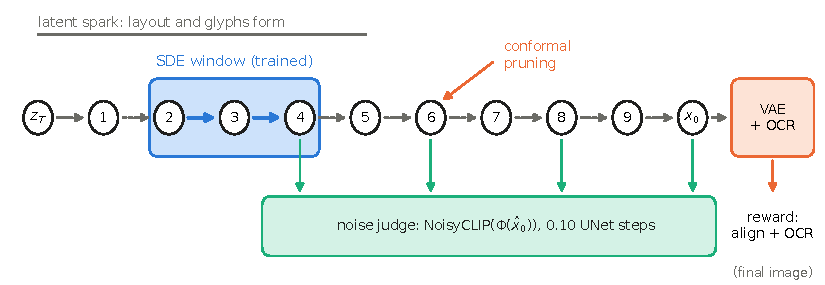
\includegraphics[width=\linewidth]{figures/overview.pdf}
  \caption{Overview. A 10-step trajectory is sampled with a deterministic sampler except inside a short stochastic (SDE)
  window in the early steps (steps 2--3 in our final text configuration), which is the only part the GRPO update trains. Alignment is judged on intermediate latents by
  NoisyCLIP on the predicted clean latent $\hat x_0$ rendered by a fixed linear map $\Phi$ (no VAE decode); the same judge can
  stop doomed rollouts early with a conformally calibrated threshold. OCR needs the decoded final image. Rewards are
  normalised within each group of images of the same prompt.}
  \label{fig:overview}
\end{figure}

%%%%%%%%%%%%%%%%%%%%%%%%%%%%%%%%%%%%%%%%%%%%%%%%%%%%%%%%%%%%%%%%%%%%%%%%%%%%%%%%%%%%%%%%%%%%%%%%%
\section{Background: Flow-GRPO}
\label{sec:flowgrpo}

\paragraph{Sampling as a Markov decision process.}
Following DDPO~\citep{black2023ddpo}, the reverse diffusion process with $T$ steps is treated as a $T$-step MDP. Given a prompt
$c$, the state at step $t$ is $(c, t, x_t)$, the action is the next latent $x_{t-1}$, and the policy is the per-step
transition $\pi_\theta(x_{t-1}\mid x_t, c)$. A reward $R(x_0, c)$ is given only at the end. Policy-gradient methods need
$\log \pi_\theta(x_{t-1}\mid x_t,c)$, so the transition must be stochastic with a tractable density.

\paragraph{From ODE to SDE.}
Flow-matching models~\citep{lipman2023flow,liu2023rectified} sample with a deterministic ODE
$\mathrm{d}x_t = v_\theta(x_t,t)\,\mathrm{d}t$, which has no density over actions. Flow-GRPO~\citep{liu2025flowgrpo} replaces it
with a reverse-time SDE with the same marginals at every $t$,
\begin{equation}
  \mathrm{d}x_t = \Big[v_\theta(x_t,t) + \frac{\sigma_t^2}{2t}\big(x_t + (1-t)\,v_\theta(x_t,t)\big)\Big]\mathrm{d}t
  + \sigma_t\,\mathrm{d}w_t ,
  \label{eq:sde}
\end{equation}
with a noise schedule $\sigma_t = a\sqrt{t/(1-t)}$. An Euler--Maruyama step of \eqref{eq:sde} is a Gaussian, so
$\log\pi_\theta$ is available in closed form, and the injected noise provides the exploration that RL needs.

\paragraph{Group-relative advantages.}
For each prompt $c$, a group of $G$ images $\{x_0^i\}_{i=1}^G$ is sampled and rewarded. The advantage of every step of
trajectory $i$ is the group-normalised reward
\begin{equation}
  \hat A^i = \frac{R(x_0^i,c) - \operatorname{mean}_j R(x_0^j,c)}{\operatorname{std}_j R(x_0^j,c)} ,
  \label{eq:adv}
\end{equation}
which removes the need for a value network. The policy maximises a clipped surrogate with a KL penalty to the reference model,
\begin{equation}
  \mathcal{J}(\theta) = \mathbb{E}\Bigg[\frac{1}{G}\sum_{i=1}^G\frac{1}{T}\sum_{t}
  \min\!\big(r_t^i(\theta)\hat A^i,\ \operatorname{clip}(r_t^i(\theta),1-\varepsilon,1+\varepsilon)\hat A^i\big)
  - \beta\, D_{\mathrm{KL}}\big(\pi_\theta\,\|\,\pi_{\mathrm{ref}}\big)\Bigg],
  \quad r_t^i(\theta)=\frac{\pi_\theta(x_{t-1}^i\mid x_t^i,c)}{\pi_{\theta_{\mathrm{old}}}(x_{t-1}^i\mid x_t^i,c)} .
  \label{eq:grpo}
\end{equation}

\paragraph{Denoising reduction.}
Flow-GRPO collects training rollouts with few steps (e.g., 10) while evaluating with the full schedule, and reports that the
learned improvements transfer. Follow-up work restricts the stochastic steps to a window
\citep{li2025mixgrpo} or weights steps by their importance \citep{he2025tempflowgrpo}, which is close in spirit to
the scheduling studied here.

%%%%%%%%%%%%%%%%%%%%%%%%%%%%%%%%%%%%%%%%%%%%%%%%%%%%%%%%%%%%%%%%%%%%%%%%%%%%%%%%%%%%%%%%%%%%%%%%%
\section{Scheduled GRPO with a noise judge}
\label{sec:method}

Our goal differs from Flow-GRPO in three ways. (1) We want few-step generation (10 steps) to be good \emph{at inference},
not only during training, so that a 10--15-step model approaches the quality of 40--50 steps. (2) We want to remove the VAE
decode and the outcome reward from as much of the RL loop as possible, by judging intermediate latents. (3) We want to spend
the policy update where it matters, i.e., on the steps that decide layout and text, and to schedule the reward over training.

\subsection{GRPO for an $\epsilon$-prediction latent diffusion model}
SD1.5 is a DDPM model with $\epsilon$-prediction, not a flow-matching model, so we obtain stochastic, density-carrying steps from
DDIM~\citep{song2021ddim} with $\eta>0$, as in DDPO. With $\bar\alpha_t$ the cumulative noise schedule and
$\xhat(x_t)=(x_t-\sqrt{1-\bar\alpha_t}\,\epsilon_\theta(x_t,t,c))/\sqrt{\bar\alpha_t}$,
\begin{equation}
  x_{t-1} = \sqrt{\bar\alpha_{t-1}}\,\xhat + \sqrt{1-\bar\alpha_{t-1}-\sigma_t^2}\;\epsilon_\theta(x_t,t,c) + \sigma_t\,\xi,
  \qquad
  \sigma_t = \eta\sqrt{\tfrac{1-\bar\alpha_{t-1}}{1-\bar\alpha_t}}\sqrt{1-\tfrac{\bar\alpha_t}{\bar\alpha_{t-1}}},
  \label{eq:ddim}
\end{equation}
with $\xi\sim\mathcal N(0,I)$, so $\pi_\theta(x_{t-1}\mid x_t,c)$ is Gaussian. We use $\eta=1$ inside a stochastic window and
$\eta=0$ (deterministic DDIM) outside it, 10 steps with classifier-free guidance 7.5, and train LoRA adapters
\citep{hu2022lora} (rank 32) on the UNet attention projections. The ``latent spark'' region $t\in[1.0,0.5]$ of a flow model
maps to the first half of the DDIM schedule (steps 1--5 of 10, timesteps $\approx 901\to 501$).

\subsection{The noise judge: NoisyCLIP on intermediate latents}
NoisyCLIP~\citep{ramos2026noisyclip} fine-tunes the vision tower of CLIP ViT-L/14~\citep{radford2021clip} to score
text--image alignment from noisy latents. The latent is rendered as a small RGB image by a fixed linear map
$\Phi:\mathbb R^4\to\mathbb R^3$ per pixel, and the score is
\begin{equation}
  s_t(c) = \cos\big(f_{\mathrm{img}}(\Phi(u_t)),\ f_{\mathrm{txt}}(c)\big),
  \label{eq:nc}
\end{equation}
where $u_t$ is the judged latent. The published judge is trained on SDXL latents with $u_t=z_t$. For SD1.5 we consider three
inputs: $z_t$ with the SDXL map (the paper's setting), the predicted clean latent $\xhat$ with the SDXL map, and $\xhat$ with an
affine map $\Phi$ fitted to SD1.5 by per-pixel least squares from the four channels of the final latent to the decoded RGB
image average-pooled to the latent resolution ($64\times64$), on 32 held-out prompts ($R^2=0.82$--$0.86$). Scoring costs one $64\times64$
projection and one CLIP forward pass, i.e., $0.10$ UNet-step equivalents per image, against $1.80$ for VAE decode + CLIP
(H200, measured). As a process reward we average the judge over steps $\{4,6,8,10\}$ of the 10-step trajectory.

\subsection{Rewards}
Prompts are of two kinds. Alignment prompts come from GenAI-Bench~\citep{li2024genaibench}. Text prompts ask for a short
quoted word (e.g., \texttt{A sign that says "OPEN"}). The reward is
\begin{equation}
  R = w_{\mathrm{al}}\, \bar s(c) + w_{\mathrm{ocr}}\,\mathrm{OCR}(x_0, y),\qquad
  \mathrm{OCR}(x_0,y) = 1-\frac{\min\big(d_{\mathrm{Lev}}(\hat y, y),\,|y|\big)}{|y|},
  \label{eq:reward}
\end{equation}
with $\bar s$ the averaged judge score, $\hat y$ the text read by PaddleOCR~\citep{li2022ppocrv3} (case- and space-insensitive,
full credit if $y$ is a substring of $\hat y$), and the OCR term applied only to text prompts. Advantages are normalised per
prompt (Eq.~\ref{eq:adv}), so only the ratio $w_{\mathrm{ocr}}/w_{\mathrm{al}}$ matters (default $80/100$). The OCR term still
needs the decoded final image, so in the mixed setting the judge removes the decode only for alignment prompts.

\subsection{Schedules}
\label{sec:schedules}
\paragraph{Reward-weight schedule.} Alignment first, text later: over the first 60 epochs $w_{\mathrm{ocr}}$ rises linearly
to its final value and $w_{\mathrm{al}}$ falls from 100 to 50. The OCR weight starts at half its final value rather than zero
(starting at zero wastes the text prompts of the first epochs).
\paragraph{Step-count schedule.} Training rollouts use 4 steps in epochs 0--19, 6 in 20--39, 8 in 40--59 and 10 from epoch 60 to the end (epoch 100), with the judge queried at
40/60/80/100\% of the current trajectory. Early epochs are 2--2.5$\times$ cheaper.
\paragraph{Step windows.} Only transitions inside a stochastic window are trained. Section~\ref{sec:res_diag} shows that, with
all steps stochastic, 57\% of the policy-gradient norm comes from the last transition, which cannot change layout or glyphs.
We therefore exclude the last transition from the update, or restrict the window to early steps.

\subsection{Conformal early pruning}
\label{sec:prune_method}
At a checkpoint step $k$, a trajectory whose judge score trails the group leader by more than a threshold $\lambda$ (in units
of the within-group standard deviation at step $k$) is stopped. $\lambda$ is chosen by conformal risk control
\citep{angelopoulos2024crc} on calibration prompts so that the expected loss, e.g., the probability of pruning the image that
would have been the best of the group, is at most $\alpha$. Savings are counted in UNet evaluations including the judge's
own cost.

%%%%%%%%%%%%%%%%%%%%%%%%%%%%%%%%%%%%%%%%%%%%%%%%%%%%%%%%%%%%%%%%%%%%%%%%%%%%%%%%%%%%%%%%%%%%%%%%%
\section{Experimental setup}
\label{sec:setup}

\paragraph{Data.} Alignment: GenAI-Bench (1{,}600 prompts), split into 1{,}440 training, 32 calibration and 128 evaluation prompts.
Text: 1{,}088 training and 128 test prompts with one- or two-word targets; training and test words are disjoint. The mixed
training set contains both training sets (2{,}528 prompts).

\paragraph{Training.} 10-step rollouts, $G=8$ images per prompt, 32 prompts (256 images) per epoch, learning rate
$3\times10^{-4}$, clip range $10^{-3}$, KL weight $\beta=0.04$ (0.01 in the final configuration), 100 epochs, single
GPU (NVIDIA H200 or A100). A 100-epoch run takes 4.5--8 GPU-hours.

\paragraph{Evaluation.} All models are evaluated with deterministic 10-step DDIM on held-out prompts:
128 GenAI-Bench prompts (CLIP-L score, PickScore~\citep{kirstain2023pickapic} as an independent judge, and accuracy against
minimally edited negative prompts) and 128 text prompts (OCR score of Eq.~\ref{eq:reward}; exact-match rate
$\mathbb{E}\,\mathbb{I}[\mathrm{OCR}(x_0,y)=1]$, which, like the reward, gives full credit whenever $y$ is a substring of the
recognised text $\hat y$; CLIP; PickScore). Seeds are fixed per image, so all comparisons with the base model are paired; we report differences with 95\%
bootstrap confidence intervals over prompts and mark significant ones with $^{*}$. In-training evaluations (512 images,
one per saved checkpoint) produced several apparent gains that did not reproduce. We therefore fix the checkpoint to report
\emph{before} looking at it (the last one) and re-evaluate it on new seeds with 8 images per prompt (1{,}024 images per set).
Only these confirmations are reported as results.

%%%%%%%%%%%%%%%%%%%%%%%%%%%%%%%%%%%%%%%%%%%%%%%%%%%%%%%%%%%%%%%%%%%%%%%%%%%%%%%%%%%%%%%%%%%%%%%%%
\section{Results}
\label{sec:results}

\subsection{Where along the trajectory are layout and text decided?}
\label{sec:res_steps}

\begin{table}[t]
  \caption{Fewer steps cost text legibility much more than alignment. Base SD1.5, deterministic DDIM, 1{,}024 images of the
  text test set (H200). CLIP saturates by 10--20 steps; at 10 steps the OCR score is 61\% of the 50-step value. CLIP is on the
  training-reward scale, $\tfrac{100}{30}\cos(f_{\mathrm{img}},f_{\mathrm{txt}})$ with CLIP ViT-L/14 (0.967 corresponds to a
  cosine of 0.290); Table~\ref{tab:main} reports the raw cosine. This table was produced with an earlier evaluation script whose
  per-image seeds differ from those of the confirmation set in Table~\ref{tab:main}, so absolute values differ slightly (e.g.,
  10-step OCR 0.118 here vs.\ 0.103 there); comparisons are only made within a table.}
  \label{tab:steps}
  \centering
  \begin{tabular}{lcccccc}
    \toprule
    Steps & 4 & 6 & 8 & 10 & 20 & 50 \\
    \midrule
    OCR score   & 0.047 & 0.065 & 0.097 & 0.118 & 0.160 & 0.193 \\
    Exact match & 0.00 & 0.01 & 0.01 & 0.02 & 0.04 & 0.04 \\
    CLIP ($\times\tfrac{100}{30}$, reward scale) & 0.819 & 0.923 & 0.953 & 0.967 & 0.977 & 0.975 \\
    \bottomrule
  \end{tabular}
\end{table}

Table~\ref{tab:steps} motivates the target: with 10 steps, SD1.5 keeps its alignment but loses 39\% of its 50-step OCR score.
To locate where text is decided, we decode the clean-image prediction $\xhat$ at every step of 10-step trajectories and score
it. The preview's OCR reaches 95\% of the final value at step 5 and 100\% at step 6. Its within-group ranking agreement with
the final OCR reward is 0.45, 0.60, 0.70 and 0.79 at steps 5, 6, 7 and 8, and steps 1--3 carry no usable ranking signal.
Text therefore forms in steps 3--5, inside the latent spark but not at its very beginning. Decoding and scoring one preview
with OCR costs about 1.4 UNet steps, so step-wise outcome rewards on decoded previews are expensive.

\subsection{Does NoisyCLIP transfer to SD1.5 latents?}
\label{sec:res_nc}

\begin{figure}[t]
  \centering
  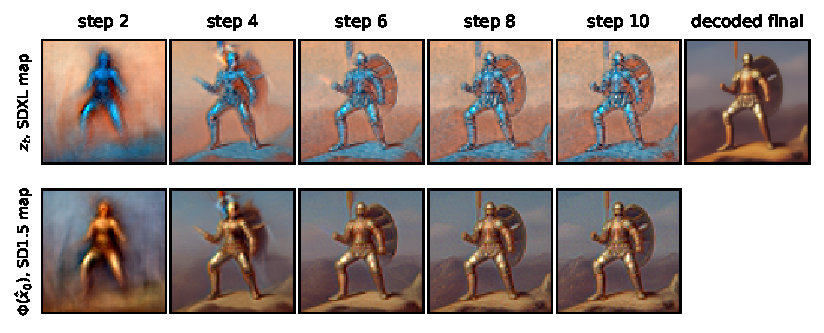
\includegraphics[width=0.9\linewidth]{figures/noisy_views.pdf}
  \caption{What the judge sees along a 10-step SD1.5 trajectory. Top: the latent rendered with NoisyCLIP's fixed SDXL colour
  map (its training input). Bottom: the predicted clean latent $\xhat$ rendered with an affine map fitted to SD1.5. The
  SD1.5 map shows the final layout from step 4--6; the SDXL map gives wrong colours on SD1.5 latents.}
  \label{fig:views}
\end{figure}

\begin{table}[t]
  \caption{Off-the-shelf NoisyCLIP needs the SD1.5 colour map and the clean-latent prediction to be useful on SD1.5. Spearman
  correlation with the final image's CLIP score (all images / within prompt) and accuracy at telling the true prompt from a
  random one. 128 held-out GenAI-Bench prompts $\times$ 4, 10 steps, $\eta=1$. Cost in UNet-step equivalents per image.}
  \label{tab:nc}
  \centering
  \small
  \begin{tabular}{lcccc}
    \toprule
    Judge (input) & Step 5 of 10 & Step 10 of 10 & Wrong-prompt acc.\ (step 5) & Cost \\
    \midrule
    NoisyCLIP ($z_t$, SDXL map; paper)        & $-0.09$ / $-0.01$ & 0.16 / 0.23 & 0.78 & 0.104 \\
    NoisyCLIP ($\xhat$, SDXL map)              & 0.09 / 0.15 & 0.17 / 0.24 & 0.98 & 0.104 \\
    NoisyCLIP ($\xhat$, SD1.5 map $\Phi$)      & 0.44 / 0.29 & 0.55 / 0.36 & 1.00 & 0.104 \\
    CLIP ($\xhat$, SD1.5 map $\Phi$)           & 0.48 / 0.29 & 0.59 / 0.29 & 0.99 & 0.096 \\
    TAESD decode + CLIP                        & 0.63 / 0.35 & 0.93 / 0.77 & 1.00 & 0.275 \\
    VAE decode + CLIP                          & 0.67 / 0.32 & 0.99 / 0.91 & 1.00 & 1.80 \\
    \bottomrule
  \end{tabular}
\end{table}

\begin{figure}[t]
  \centering
  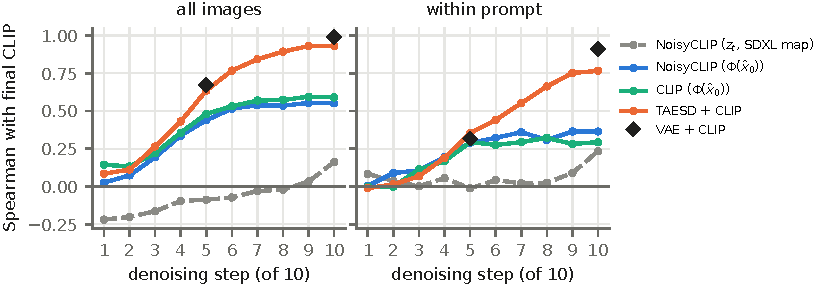
\includegraphics[width=\linewidth]{figures/nc_steps.pdf}
  \caption{How well each judge, applied at an intermediate step, predicts the CLIP score of the final image (Spearman over all
  images, left, and within prompt, right; same data as Table~\ref{tab:nc}). The VAE decode was scored only at steps 5 and 10.
  NoisyCLIP on raw SD1.5 latents carries almost no signal; on $\Phi(\xhat)$ it tracks plain CLIP on the same view.}
  \label{fig:nc_steps}
\end{figure}

Table~\ref{tab:nc} and Figure~\ref{fig:nc_steps} show that the published judge, applied to SD1.5 noisy latents as in its
paper, is close to chance at mid-trajectory. NoisyCLIP is trained on SDXL latents, whose channels encode colour differently (Figure~\ref{fig:views}).
Feeding it the clean-latent prediction rendered with an SD1.5 map recovers a useful signal (0.44 at step 5), on par with plain
CLIP on the same image, at 6\% of the decode cost. A tiny decoder (TAESD) is more accurate at 2.6$\times$ the cost of the judge
(0.275 vs.\ 0.104 UNet-step equivalents). Appendix~\ref{app:compute} collects all cost measurements. We
use NoisyCLIP on $\Phi(\xhat)$ as the alignment judge in all NoisyCLIP runs.

\subsection{How much rollout compute does early pruning save?}
\label{sec:res_prune}
With $G=4$ and the risk ``the best image of the group is pruned'' at $\alpha=0.1$, conformal pruning with the NoisyCLIP judge
saves 7\% of UNet compute (TAESD: 9\%, at step 6; VAE decoding: $-7\%$, because decoding costs more than it saves). Pruning at
random at step 1 saves about 9\% at the same risk. At $\alpha=0.2$ the judge saves 14--16\%, TAESD 17\%, random pruning
about 18\%. The guarantee holds in all cases (test risk $\approx\alpha$ over 40 random calibration/test splits), but with an
off-the-shelf judge pruning does not beat random selection. Two factors limit the savings: before step 4--5 no judge ranks
images reliably, and a trajectory pruned at step 6 of 10 saves only 40\% of its steps.

\subsection{GRPO with the noise judge: prompt alignment and text}
\label{sec:res_grpo}

\begin{table}[t]
  \caption{Confirmations on new seeds (1{,}024 images per set, paired with the base model at 10 steps; differences with
  $^{*}$ have a 95\% bootstrap CI excluding zero). For the scheduled runs and the final configuration the last checkpoint
  was fixed before evaluation; for the ORM and distilled-judge runs the best in-training checkpoint was confirmed, which can
  only favour them. Only the
  NoisyCLIP run improves alignment on both judges. Among the standard-budget runs only the weight schedule with the distilled
  judge improves OCR, at the edge of significance; the 10$\times$-volume run lifts OCR in two independent training seeds, to
  the 50-step level for seed 1 and the 20-step level for seed 2.}
  \label{tab:main}
  \centering
  \small
  \setlength{\tabcolsep}{4pt}
  \begin{tabular}{lcccccc}
    \toprule
    & \multicolumn{2}{c}{Alignment prompts} & \multicolumn{4}{c}{Text prompts} \\
    \cmidrule(r){2-3}\cmidrule(l){4-7}
    Model & CLIP & PickScore & CLIP & PickScore & OCR & Exact \\
    \midrule
    Base, 10 steps (absolute)  & 0.2828 & 0.8156 & 0.2872 & 0.7746 & 0.1025 & 0.013 \\
    Base, 20 steps             & $+0.0010$ & $+0.0075$\sig & $+0.0047$\sig & $+0.0114$\sig & $+0.0487$\sig & $+0.022$\sig \\
    Base, 50 steps             & $-0.0001$ & $+0.0106$\sig & $+0.0055$\sig & $+0.0166$\sig & $+0.0787$\sig & $+0.024$\sig \\
    \midrule
    ORM: CLIP on decoded image & $+0.0001$ & $-0.0020$\sig & $+0.0004$ & $+0.0011$\sig & $+0.0038$ & $+0.003$ \\
    Distilled latent judge$^{\dagger}$  & $-0.0001$ & $-0.0008$ & $+0.0014$ & $+0.0004$ & $+0.0045$ & $+0.006$ \\
    \quad + weight schedule$^{\dagger}$ & $+0.0004$ & $+0.0000$ & $+0.0013$ & $+0.0021$\sig & $+0.0135$\sig & $+0.009$ \\
    \quad + step schedule$^{\dagger}$   & $-0.0002$ & $-0.0003$ & $-0.0003$ & $+0.0012$\sig & $+0.0000$ & $+0.005$ \\
    \textbf{NoisyCLIP + weight schedule + fixes} & $\mathbf{+0.0014}$\sig & $\mathbf{+0.0015}$\sig & $\mathbf{+0.0069}$\sig &
      $\mathbf{+0.0035}$\sig & $-0.0072$ & $+0.010$ \\
    \midrule
    Differentiable OCR reward (Sec.~\ref{sec:res_diag}) & $-0.1075$\sig & $-0.1259$\sig & $-0.0569$\sig & $-0.0728$\sig & $-0.0522$\sig & $-0.003$ \\
    \textbf{Long OCR run, 256k images}, seed 1 (Sec.~\ref{sec:res_diag}) & $+0.0002$ & $-0.0013$\sig & $\mathbf{+0.0164}$\sig & $\mathbf{+0.0120}$\sig & $\mathbf{+0.0850}$\sig & $\mathbf{+0.027}$\sig \\
    \textbf{Long OCR run, 256k images}, seed 2 & $-0.0001$ & $-0.0011$ & $+0.0081$\sig & $+0.0069$\sig & $+0.0473$\sig & $+0.012$ \\
    \bottomrule
  \end{tabular}
  \\[2pt]
  {\footnotesize $^{\dagger}$Earlier runs whose alignment reward was a CLIP-distilled latent judge (Appendix~\ref{app:distilled})
  instead of NoisyCLIP; ORM and distilled-judge runs: checkpoint at epoch 60, others epoch 100.}
\end{table}

Table~\ref{tab:main} lists every confirmed run. The final configuration (NoisyCLIP judge on $\Phi(\xhat)$ at steps 4/6/8/10,
OCR weight $40\to80$ and alignment weight $100\to50$ over 60 epochs, last transition excluded from the update, $\beta=0.01$, one
optimiser step of 256 images per epoch) is the only run that improves alignment on both judges, including PickScore, which is
not used in training. It also improves the text-prompt CLIP score beyond the base model at 20 steps
($+0.0069$ vs.\ $+0.0047$). These gains are small in absolute terms; PickScore remains well below the 20- and 50-step levels. The
outcome-reward baseline, which decodes every image, does not improve alignment and slightly lowers PickScore. Note that this
configuration changes several things at once relative to the earlier runs: the judge, the weight schedule, and the stability
fixes motivated by the diagnosis in Section~\ref{sec:res_diag} (excluding the last transition, lower $\beta$, one large update per
epoch) were bundled together, so Table~\ref{tab:main} does not attribute the gain to any single change.

OCR, in contrast, is not improved by any configuration in a way that survives confirmation, except the weight-scheduled
run with the distilled judge ($+0.0135$, CI $[+0.0007, +0.0269]$), which recovers only a quarter of the gap to 20 steps.
In-training evaluations repeatedly suggested OCR gains of $+0.02$--$0.03$ that vanished on new seeds; the PRM run, for
instance, showed $+0.026^{*}$ in training and $+0.005$ on confirmation, a selection effect from choosing the best of 12
checkpoints.

\subsection{Why does the OCR reward not teach legible text?}
\label{sec:res_diag}

\paragraph{The reward signal is present.} On text prompts, the OCR score varies strongly within a group (standard deviation
0.24--0.28, range 0.63--0.71); 72--78\% of groups contain an image with OCR $\ge0.5$ and 41--50\% contain an exact match. OCR
explains 80--88\% of the within-group reward variance, and the advantage correlates 0.97--0.99 with it. The common explanation
for failed RL on text, that groups contain no good sample, does not apply to short targets.

\paragraph{The gradient signal is not.} Let $g_i = \hat A^i\nabla_\theta\sum_t\log\pi_\theta(x^i_{t-1}\mid x^i_t,c)$ be
the per-image contribution to the policy gradient, with mean $\mu$ and covariance $\Sigma$ over the sampling distribution. We
define the per-image signal-to-noise ratio $\rho^2=\|\mu\|^2/\operatorname{tr}\Sigma$; an update over $B$ images then has
$\mathrm{SNR}\approx\sqrt{B\rho^2}$. Naive estimates of $\|\mu\|$ from one batch are inflated by noise (a pure-noise batch of
size $N$ has $\|\bar g\|^2\approx\operatorname{tr}\Sigma/N$), so we estimate $\|\mu\|^2$ without bias from cross-products of
gradient sums over disjoint folds, $\mathbb E\langle S_f,S_{f'}\rangle=n_fn_{f'}\|\mu\|^2$ for $f\neq f'$, with jackknife
standard errors. On 64 text prompts $\times$ 8 images:

\begin{table}[h]
  \caption{Per-image policy-gradient signal under different sampling schemes (base model, 64 text prompts $\times$ 8,
  paired seeds). No variant raises the signal; all are within noise of each other and of zero.}
  \label{tab:snr}
  \centering
  \small
  \begin{tabular}{lccc}
    \toprule
    Sampling variant & $\rho^2$ ($\pm$ s.e.) & SNR at 256 images (95\% CI) & Within-group OCR std \\
    \midrule
    Own $z_T$, all steps 1--8 (current) & $1.3\times10^{-4}\pm1.0\times10^{-4}$ & $+0.19$ $[-0.12,+0.29]$ & 0.270 \\
    Shared $z_T$, all steps          & $-1.0\times10^{-4}\pm1.2\times10^{-4}$ & $-0.16$ $[-0.29,+0.18]$ & 0.253 \\
    Own $z_T$, window steps 1--4     & $1.0\times10^{-4}\pm1.2\times10^{-4}$ & $+0.16$ $[-0.19,+0.30]$ & 0.269 \\
    Shared $z_T$, window steps 1--4  & $0.0\pm1.7\times10^{-4}$ & $+0.01$ $[-0.29,+0.30]$ & 0.227 \\
    Shared $z_T$, window steps 2--3  & $1.6\times10^{-4}\pm1.0\times10^{-4}$ & $+0.20$ $[-0.09,+0.30]$ & 0.175 \\
    \bottomrule
  \end{tabular}
\end{table}

With $\rho^2\approx1.5\times10^{-4}$, one update needs $1/\rho^2\approx6{,}000$--$10{,}000$ images before signal equals noise,
whereas an update uses 256. Over a whole 100-epoch run (25{,}600 images), the accumulated signal is only
$\sqrt{25{,}600\cdot1.3\times10^{-4}}\approx1.8$ times the noise. This explains small, non-reproducible OCR gains without
any fault in the reward or the hyperparameters. Sharing the initial noise $z_T$ within a group barely reduces the OCR spread
(0.270$\to$0.253), so the stochastic steps, not $z_T$, decide whether the text comes out, and $z_T$ is not the hidden source of
noise.

\begin{figure}[t]
  \centering
  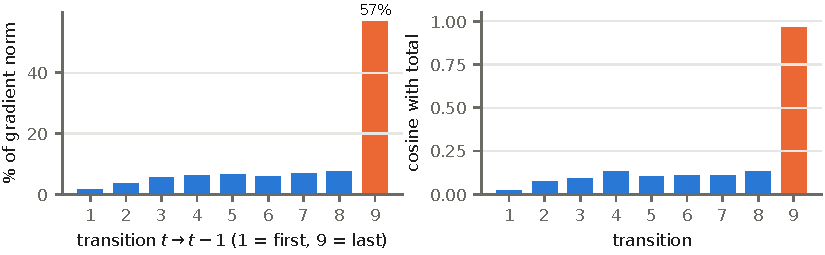
\includegraphics[width=\linewidth]{figures/grad_share.pdf}
  \caption{Where the policy gradient comes from (base model, all 9 transitions stochastic, 384 images). Left: share of the
  gradient norm per transition. Right: cosine between each transition's gradient and the total. The last transition, which
  only sharpens details, dominates both.}
  \label{fig:grad_share}
\end{figure}

\paragraph{Gradient and KL are dominated by the last step.} With all steps stochastic, 57\% of the policy-gradient norm comes
from the last transition ($t=101\to1$; Figure~\ref{fig:grad_share}). The reason is the Gaussian form of Eq.~\ref{eq:ddim}: with mean $m_\theta$ and
$x_{t-1}=m_{\theta_{\mathrm{old}}}+\sigma_t\xi$,
\begin{equation}
  \nabla_\theta\log\pi_\theta(x_{t-1}\mid x_t,c)=\sigma_t^{-2}\,(x_{t-1}-m_\theta)^{\top}\nabla_\theta m_\theta
  =\sigma_t^{-1}\,\xi^{\top}\nabla_\theta m_\theta=\mathcal O(\sigma_t^{-1}),
  \qquad
  D_{\mathrm{KL}}\big(\pi_\theta\|\pi_{\mathrm{ref}}\big)=\frac{\|m_\theta-m_{\mathrm{ref}}\|^2}{2\sigma_t^2}=\mathcal O(\sigma_t^{-2}),
  \label{eq:sigma}
\end{equation}
at $\theta\approx\theta_{\mathrm{old}}$, and $\sigma_t$ of Eq.~\ref{eq:ddim} is by far the smallest at the last transition, where
$1-\bar\alpha_{t-1}\to0$. This transition only sharpens details that are already fixed. Its gradient is nearly parallel to the total
(cosine 0.96), while every other transition contributes 1.5--8\%. 92\% of the KL-penalty gradient also comes from this
transition, and at $\beta=0.04$ the KL gradient is 0.7--1.2$\times$ the policy gradient by the end of training. This
motivated excluding the last transition and lowering $\beta$ in the final configuration.

\paragraph{Remedy 1: a differentiable OCR reward.} Backpropagating a differentiable reward through the sampler
\citep{clark2024draft,prabhudesai2023alignprop,xu2023imagereward} removes the sampling noise from the gradient. We used the
negative log-likelihood of the target under TrOCR~\citep{li2023trocr} (large, scene-text) on PaddleOCR line crops, plus a CLIP
text-match term, and backpropagated through the last 8 of 10 deterministic DDIM steps and the VAE decoder with gradient
checkpointing (600 updates of 8 images). Before training, no differentiable proxy agreed with PaddleOCR within a prompt
(best Spearman 0.17). During training the PaddleOCR score on training images halved ($0.245\to0.125$) while only the CLIP term
rose; on new seeds both text and image quality collapsed (Table~\ref{tab:main}). The proxy is hacked.

\begin{figure}[t]
  \centering
  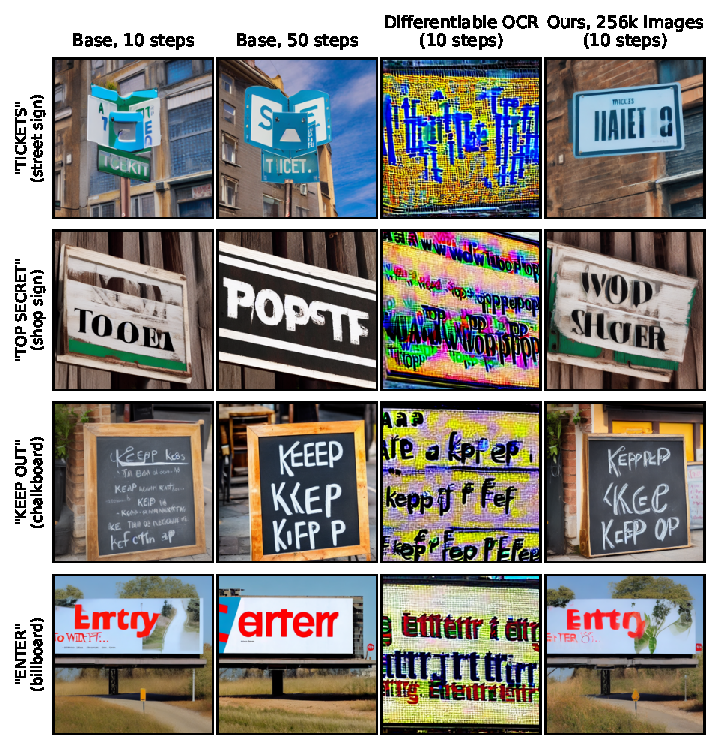
\includegraphics[width=0.78\linewidth]{figures/qualitative.pdf}
  \caption{Same prompts and initial noise for all models (four of the first eight text test prompts, first image each; not
  selected by score). The differentiable OCR reward collapses image quality. The 256k-image GRPO run writes larger, cleaner
  glyphs at 10 steps; it sometimes repeats the word (``KEEP OUT'' row), but such repetitions are rare in OCR terms
  (Table~\ref{tab:robust}). The misspellings show that legibility is far from solved.}
  \label{fig:qual}
\end{figure}

\paragraph{Remedy 2: volume.} If per-image signal cannot be raised, the number of images must be. We trained on text prompts
only, with a 2-step stochastic window (steps 2--3, shared $z_T$), which cuts training cost per image about 4$\times$ at the same
$\rho^2$, using 512 images per update and 500 updates (256k images, 10$\times$ the previous run, 23 H200-hours). The OCR score on
training images rose steadily from 0.253 (epochs 0--49) to 0.364 (epochs 300--349), the first sustained rise in any run.
On held-out words, the in-training evaluation shows OCR above the base model at every checkpoint
(Figure~\ref{fig:ocr_curves}a). The pre-chosen final checkpoint, re-evaluated on new seeds (Table~\ref{tab:main}), reaches an OCR
score of 0.188 against 0.103 for the base model at 10 steps ($+0.085$, CI $[+0.064,+0.106]$) and 0.181 at 50 steps; the
difference to 50 steps is not significant ($+0.006$, CI $[-0.018,+0.030]$), and exact matches (4.0\% vs.\ 3.7\%) are also at the
50-step level. Text-prompt PickScore improves by $+0.012$, the gain of 20 sampling steps. The cost is a small drop in alignment
PickScore ($-0.0013$, CI upper bound $0.0000$) with unchanged CLIP and negative-prompt accuracy, although no alignment prompts
were trained.

\paragraph{A second training seed.} We repeated the run with a different training seed (sampling noise, prompt order and
initial noise). The gain reproduces but is smaller: OCR 0.150 ($+0.047$, CI $[+0.031,+0.064]$), at the 20-step level
($-0.001$ vs.\ 20 steps, n.s.) and below the 50-step level ($-0.031^{*}$); exact matches $+1.2$\,pp (CI $[0.0, +2.4]$); text-prompt
CLIP $+0.008^{*}$ and PickScore $+0.007^{*}$; alignment unchanged. The two seeds differ significantly ($+0.038^{*}$). Their
in-training curves (Figure~\ref{fig:ocr_curves}a) are similar up to epoch 200 and then fluctuate by about $\pm0.03$ between
checkpoints, so part of the seed-1 result is a favourable final checkpoint. Averaged over seeds, the 256k-image run adds
$+0.066$ OCR at 10 steps, closing about 85\% of the gap between 10 and 50 steps of the base model.

\begin{figure}[t]
  \centering
  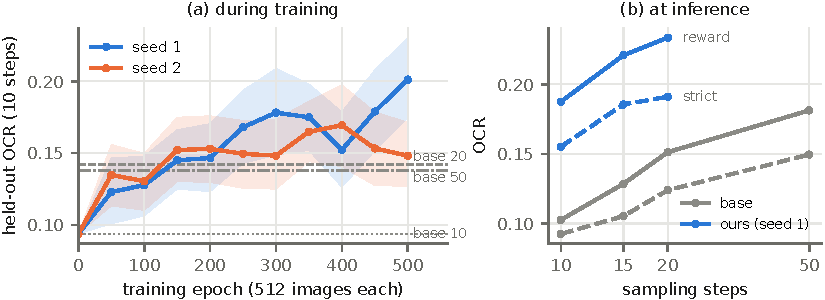
\includegraphics[width=\linewidth]{figures/ocr_curves.pdf}
  \caption{(a) Held-out OCR at 10 steps during the 256k-image run, two training seeds (in-training evaluation: 128 test words
  $\times$ 4 images; bands: 95\% bootstrap CI of the paired difference to the base model, drawn around the base value). Dashed
  lines: base model at 10/20/50 steps on the same images (on this set the 20- and 50-step values are within noise of each
  other). (b) OCR of seed 1's final checkpoint when sampled with more steps (confirmation seeds, 1{,}024 images per point;
  solid: training reward, dashed: strict OCR without substring credit).}
  \label{fig:ocr_curves}
\end{figure}

\paragraph{Is the gain an artefact of the OCR reward?} (Seed 1.) Figure~\ref{fig:qual} suggests that the model sometimes writes the word
several times, and the reward gives full credit when the target is a substring of the recognised text. We regenerated the
confirmation images and re-scored them with stricter metrics (Table~\ref{tab:robust}). The gain survives without substring
credit (strict OCR $+0.063$), at least one detected line reads exactly the target four times as often, and a second recogniser
(TrOCR-large, reading the same PaddleOCR line crops) reads the exact target 3.5$\times$ as often. The target occurs twice or more
in only 0.3\% of images (base: 0.0\%), and the number of detected text lines is unchanged (2.5 vs.\ 2.5), so repetition does not
explain the gain; the visible repetitions are mostly misspelled and earn no extra credit. The improvement also transfers to
more sampling steps: at 20 steps the model exceeds the 50-step base model on every metric (strict OCR $+0.042^{*}$;
Figure~\ref{fig:ocr_curves}b).
A fully independent OCR engine (EasyOCR, with its own detector and recogniser; paired run on an A100) confirms the gain: at 10 steps, $+0.058^{*}$ with the substring rule, $+0.046^{*}$ strict, and an exactly read line in 1.4\% vs.\ 0.5\% of images$^{*}$, with no detected repetition in either model. Against the 50-step base model, EasyOCR finds our 10-step model statistically equal (strict $-0.011$, n.s.) and our 20-step model better (strict $+0.037^{*}$). At 15 and 20 steps the gain over the base model at the same step count is $+0.067^{*}$ and $+0.062^{*}$ (strict).

\begin{table}[t]
  \caption{The OCR gain under stricter metrics (seed-1 model; same seeds as Table~\ref{tab:main}, 1{,}024 images per row, H200). Strict: no
  substring credit (extra text is penalised). Line exact: some detected line equals the target. TrOCR exact: a second
  recogniser reads the target exactly on some line crop. Repeat: target occurs $\ge2$ times. $^{*}$: paired 95\% CI vs.\ base at
  the same number of steps excludes zero.}
  \label{tab:robust}
  \centering
  \small
  \setlength{\tabcolsep}{4pt}
  \begin{tabular}{lcccccc}
    \toprule
    Model, steps & OCR (reward) & Strict OCR & Line exact & Best-line score & TrOCR exact & Repeat \\
    \midrule
    Base, 10   & 0.103 & 0.092 & 0.007 & 0.314 & 0.019 & 0.000 \\
    Ours, 10   & 0.187\sig & 0.155\sig & 0.027\sig & 0.457\sig & 0.067\sig & 0.003 \\
    Base, 15   & 0.128 & 0.105 & 0.010 & 0.358 & 0.026 & 0.000 \\
    Ours, 15   & 0.221\sig & 0.186\sig & 0.040\sig & 0.495\sig & 0.069\sig & 0.004 \\
    Base, 20   & 0.151 & 0.124 & 0.016 & 0.370 & 0.042 & 0.001 \\
    Ours, 20   & 0.234\sig & 0.191\sig & 0.040\sig & 0.494\sig & 0.074\sig & 0.001 \\
    Base, 50   & 0.181 & 0.149 & 0.026 & 0.391 & 0.051 & 0.002 \\
    \bottomrule
  \end{tabular}
\end{table}

%%%%%%%%%%%%%%%%%%%%%%%%%%%%%%%%%%%%%%%%%%%%%%%%%%%%%%%%%%%%%%%%%%%%%%%%%%%%%%%%%%%%%%%%%%%%%%%%%
\section{Related work}
\label{sec:related}

\paragraph{RL for diffusion models.} DDPO~\citep{black2023ddpo} and DPOK~\citep{fan2023dpok} cast denoising as an MDP and
optimise rewards with policy gradients. Flow-GRPO~\citep{liu2025flowgrpo} and DanceGRPO~\citep{xue2025dancegrpo} extend GRPO
\citep{shao2024deepseekmath} to flow models; MixGRPO~\citep{li2025mixgrpo} and TempFlow-GRPO~\citep{he2025tempflowgrpo}
restrict or reweight the stochastic steps. Direct reward backpropagation (ReFL~\citep{xu2023imagereward},
DRaFT~\citep{clark2024draft}, AlignProp~\citep{prabhudesai2023alignprop}) is sample-efficient but requires a differentiable
reward and is prone to reward hacking, which we observe for OCR.

\paragraph{Process and latent rewards.} Process reward models score intermediate steps of a solution
\citep{lightman2023verify}. For diffusion, step-aware preference optimisation~\citep{liang2024spo} and latent reward models
\citep{zhang2025lpo} judge noisy latents for step-level preference learning. NoisyCLIP~\citep{ramos2026noisyclip} aligns prompts
with noisy latents directly; we use it as an RL process reward and test its transfer across latent spaces.

\paragraph{Fewer sampling steps and text rendering.} Step reduction is usually obtained by distillation
\citep{salimans2022progressive,song2023consistency,luo2023lcm}; we instead ask whether RL can make a fixed few-step sampler
better. Legible text is typically improved with glyph conditioning or specialised architectures
\citep{chen2023textdiffuser,yang2023glyphcontrol}; we study it as a pure reward-learning problem.

\paragraph{Early stopping with guarantees.} Conformal risk control~\citep{angelopoulos2024crc} provides distribution-free
bounds on expected loss, which we use to calibrate the pruning threshold.

%%%%%%%%%%%%%%%%%%%%%%%%%%%%%%%%%%%%%%%%%%%%%%%%%%%%%%%%%%%%%%%%%%%%%%%%%%%%%%%%%%%%%%%%%%%%%%%%%
\section{Limitations}
\label{sec:limits}
All experiments use one model (SD1.5) and one resolution. Only the final text configuration was trained with two seeds, and
their gains differ significantly ($+0.085$ vs.\ $+0.047$); all other configurations have a single training seed, and the
confirmed alignment gains are small. The robustness checks with stricter metrics and other OCR engines were run on seed 1 only. The off-the-shelf judge was trained on SDXL latents and only partly transfers; a judge trained for SD1.5
latents would likely change the pruning and process-reward results. The OCR reward relies on a CPU OCR engine whose partial
credit is itself noisy (garbage text that shares a few characters with the target receives credit). Our gradient-signal
measurements are made on the base and a few trained models with 512 images, so their confidence intervals are wide; they bound
the signal rather than measure it precisely.

\paragraph{Future work.} (i) Flow-matching models with 16-channel latents (e.g., SD3.5) have straighter trajectories, so their
clean-latent previews in the latent spark should be more informative; a noise judge trained for those latents could make the
process reward and early pruning pay off where an SDXL-trained judge on SD1.5 does not. (ii) The OCR result suggests that the
useful lever is the per-image gradient signal $\rho^2$. A localised latent judge for glyphs (e.g., pooled over the text region
via cross-attention maps) could give a denser, lower-variance reward than a global OCR score; whether it raises $\rho^2$ above
$10^{-4}$ is an open, measurable question with the estimator of Section~\ref{sec:res_diag}.

\section{Conclusion}
\label{sec:conclusion}
Scheduling GRPO around a noise judge on latents is viable for a latent diffusion model: the judge removes the decode from the
alignment reward at 6\% of its cost, and GRPO with it produces a small alignment gain that survives an independent check on new
seeds. For legible text, the bottleneck is not the reward but the estimator: the per-image policy-gradient signal of an OCR
reward is about $10^{-4}$ of its variance, which neither sampling changes nor a differentiable proxy can fix. Measuring this
signal tells how many images a run needs; supplying them, with a cheap 2-step window over the steps where text forms, makes a
10-step SD1.5 model render text at the level of the base model with 20 to 50 steps (two training seeds), i.e., with 2--5$\times$
fewer denoising steps, and the trained model at 20 steps surpasses the base model at 50.

\begin{ack}
\tbd{Acknowledgements and funding (hidden in the anonymous submission).}
\end{ack}

\bibliographystyle{abbrvnat}
\bibliography{references}

%%%%%%%%%%%%%%%%%%%%%%%%%%%%%%%%%%%%%%%%%%%%%%%%%%%%%%%%%%%%%%%%%%%%%%%%%%%%%%%%%%%%%%%%%%%%%%%%%
\appendix

\section{Distilled latent judge used in earlier runs}
\label{app:distilled}
Before the off-the-shelf NoisyCLIP checkpoint was available for SD1.5 experiments, earlier runs (marked $^{\dagger}$ in
Table~\ref{tab:main}) used a CLIP ViT-L/14 vision tower with LoRA (rank 16) and a timestep embedding, trained on
$\Phi(\xhat_t)$ from 10-step $\eta=1$ trajectories of 1{,}440 GenAI-Bench training prompts to predict the CLIP embedding of the
final decoded image. Its Spearman correlation with the final CLIP score at steps 4/5/6 of 10 was 0.68/0.80/0.86 on held-out
prompts, at 0.16 UNet-step equivalents per image. We report it only to make the earlier runs reproducible.

\section{Compute and latency}
\label{app:compute}

\begin{table}[h]
  \caption{Cost per image on one NVIDIA H200 unless noted. UNet step = one guided UNet evaluation (17.4\,ms). Inference latency
  is derived from the measured per-call costs (UNet steps + VAE decode), not measured end to end.}
  \label{tab:compute}
  \centering
  \small
  \begin{tabular}{llcc}
    \toprule
    & Operation & ms / image & UNet-step equiv. \\
    \midrule
    \multirow{5}{*}{Scoring} & NoisyCLIP judge ($\Phi(\xhat)$ + CLIP) & 1.8 & 0.104 \\
    & CLIP on $\Phi(\xhat)$ & 1.7 & 0.096 \\
    & TAESD decode + CLIP & 4.8 & 0.275 \\
    & VAE decode + CLIP & 31.3 & 1.80 \\
    & PaddleOCR det.\ + rec.\ (CPU) & $\approx$50 & $\approx$2.9 \\
    \midrule
    \multirow{3}{*}{Training} & Rollout + rewards, 10 steps (256k-image run) & 215 & -- \\
    & Policy update, 2-step window (256k-image run) & 100 & -- \\
    & Policy update, 8 transitions (A100, final NoisyCLIP run) & 785 & -- \\
    \midrule
    \multirow{2}{*}{Inference} & 10 steps + VAE decode & $\approx$204 & 10 + decode \\
    & 50 steps + VAE decode & $\approx$900 & 50 + decode \\
    \bottomrule
  \end{tabular}
\end{table}

A 10-step model is therefore about 4.4$\times$ faster per image at inference than the 50-step base model and about
1.9$\times$ faster than the 20-step one ($\approx$380\,ms). The 2-step window trains
2 of the 8 transitions per image, i.e., about 4$\times$ fewer UNet backward passes than training all transitions.

\section{Additional training details}
\label{app:details}
\begin{table}[h]
  \caption{Hyperparameters of the two final configurations. Shared by all GRPO runs unless stated: SD1.5
  (\texttt{runwayml/stable-diffusion-v1-5}), 512$\times$512, classifier-free guidance 7.5, 10-step DDIM, LoRA rank 32 and
  $\alpha=64$ on the attention projections (\texttt{to\_q}, \texttt{to\_k}, \texttt{to\_v}, \texttt{to\_out}) of the UNet, AdamW
  (weight decay $10^{-4}$), bf16, PPO clip range $10^{-3}$, advantages clipped to $[-5,5]$, gradient-norm clip 1.0, one inner epoch,
  KL reference = the base model.}
  \label{tab:hparams}
  \centering
  \small
  \begin{tabular}{lcc}
    \toprule
    & NoisyCLIP + weight schedule + fixes & Long OCR run (256k images) \\
    \midrule
    Prompts & 1{,}440 GenAI-Bench + 1{,}088 text & 1{,}088 text \\
    Alignment reward & NoisyCLIP on $\Phi(\xhat)$, steps 4/6/8/10 & same \\
    Reward weights (align / OCR) & $100\to50$ / $40\to80$ over 60 epochs & 100 / 80 \\
    Stochastic steps ($\eta=1$) & all 10 & steps 2--3 only \\
    Trained transitions & first 8 (last excluded) & 2 \\
    Initial noise $z_T$ in a group & independent & shared \\
    Group size $G$ & 8 & 8 \\
    Images per optimiser step & 256 (32 prompts) & 512 (64 prompts) \\
    Optimiser steps (epochs) & 100 & 500 \\
    Learning rate & $3\times10^{-4}$ & $3\times10^{-4}$ \\
    KL coefficient $\beta$ & 0.01 & 0.01 \\
    Training seeds & 1 & 2 \\
    Hardware, wall-clock & 1$\times$A100-40GB, 8.3\,h & 1$\times$H200, 22.6\,h per seed \\
    \bottomrule
  \end{tabular}
\end{table}

\paragraph{Prompts.} Text prompts are generated from templates that place a 1--2-word target in quotes in a scene, e.g.,
\emph{A neon sign that says ``PUSH'' glowing on a brick wall at night}; the 1{,}088 training and 128 test prompts use disjoint
words. Alignment prompts are the GenAI-Bench prompts~\citep{li2024genaibench}; the 128 evaluation and 32 $\Phi$-calibration
prompts are excluded from training.

\paragraph{OCR.} PaddleOCR 2.8.1 (PP-OCRv3 detector and English recogniser) on CPU, without angle classification. The
recognised lines are concatenated, spaces removed and lower-cased; the score is $1-\mathrm{Lev}(\hat y,y)/|y|$ (clipped at 0),
or 1 if $y$ is a substring of $\hat y$. The robustness checks use TrOCR-large (scene-text) with greedy decoding and EasyOCR
(English, CRAFT detector) with the same normalisation.

\paragraph{Evaluation.} In-training evaluations: 128 held-out prompts per set $\times$ 4 images, 10-step deterministic DDIM,
fixed per-image seeds. Confirmations: the same prompts $\times$ 8 images with a different seed set (1{,}024 images per set), on the
same GPU type as the base references (H200), because the same seed gives different images on different GPU types. Confidence
intervals: 2{,}000 bootstrap resamples over prompts of the paired per-prompt differences.

\newpage
\section*{NeurIPS Paper Checklist}

%%% BEGIN INSTRUCTIONS %%%
The checklist is designed to encourage best practices for responsible machine learning research, addressing issues of reproducibility, transparency, research ethics, and societal impact. Do not remove the checklist: {\bf The papers not including the checklist will be desk rejected.} The checklist should follow the references and follow the (optional) supplemental material.  The checklist does NOT count towards the page
limit. 

Please read the checklist guidelines carefully for information on how to answer these questions. For each question in the checklist:
\begin{itemize}
    \item You should answer \answerYes{}, \answerNo{}, or \answerNA{}.
    \item \answerNA{} means either that the question is Not Applicable for that particular paper or the relevant information is Not Available.
    \item Please provide a short (1--2 sentence) justification right after your answer (even for \answerNA). 
   % \item {\bf The papers not including the checklist will be desk rejected.}
\end{itemize}

{\bf The checklist answers are an integral part of your paper submission.} They are visible to the reviewers, area chairs, senior area chairs, and ethics reviewers. You will also be asked to include it (after eventual revisions) with the final version of your paper, and its final version will be published with the paper.

The reviewers of your paper will be asked to use the checklist as one of the factors in their evaluation. While \answerYes{} is generally preferable to \answerNo{}, it is perfectly acceptable to answer \answerNo{} provided a proper justification is given (e.g., error bars are not reported because it would be too computationally expensive'' or ``we were unable to find the license for the dataset we used''). In general, answering \answerNo{} or \answerNA{} is not grounds for rejection. While the questions are phrased in a binary way, we acknowledge that the true answer is often more nuanced, so please just use your best judgment and write a justification to elaborate. All supporting evidence can appear either in the main paper or the supplemental material, provided in appendix. If you answer \answerYes{} to a question, in the justification please point to the section(s) where related material for the question can be found.

IMPORTANT, please:
\begin{itemize}
    \item {\bf Delete this instruction block, but keep the section heading ``NeurIPS Paper Checklist"},
    \item  {\bf Keep the checklist subsection headings, questions/answers and guidelines below.}
    \item {\bf Do not modify the questions and only use the provided macros for your answers}.
\end{itemize} 
 

%%% END INSTRUCTIONS %%%


\begin{enumerate}

\item {\bf Claims}
    \item[] Question: Do the main claims made in the abstract and introduction accurately reflect the paper's contributions and scope?
    \item[] Answer: \answerTODO{} % Replace by \answerYes{}, \answerNo{}, or \answerNA{}.
    \item[] Justification: \justificationTODO{}
    \item[] Guidelines:
    \begin{itemize}
        \item The answer \answerNA{} means that the abstract and introduction do not include the claims made in the paper.
        \item The abstract and/or introduction should clearly state the claims made, including the contributions made in the paper and important assumptions and limitations. A \answerNo{} or \answerNA{} answer to this question will not be perceived well by the reviewers. 
        \item The claims made should match theoretical and experimental results, and reflect how much the results can be expected to generalize to other settings. 
        \item It is fine to include aspirational goals as motivation as long as it is clear that these goals are not attained by the paper. 
    \end{itemize}

\item {\bf Limitations}
    \item[] Question: Does the paper discuss the limitations of the work performed by the authors?
    \item[] Answer: \answerTODO{} % Replace by \answerYes{}, \answerNo{}, or \answerNA{}.
    \item[] Justification: \justificationTODO{}
    \item[] Guidelines:
    \begin{itemize}
        \item The answer \answerNA{} means that the paper has no limitation while the answer \answerNo{} means that the paper has limitations, but those are not discussed in the paper. 
        \item The authors are encouraged to create a separate ``Limitations'' section in their paper.
        \item The paper should point out any strong assumptions and how robust the results are to violations of these assumptions (e.g., independence assumptions, noiseless settings, model well-specification, asymptotic approximations only holding locally). The authors should reflect on how these assumptions might be violated in practice and what the implications would be.
        \item The authors should reflect on the scope of the claims made, e.g., if the approach was only tested on a few datasets or with a few runs. In general, empirical results often depend on implicit assumptions, which should be articulated.
        \item The authors should reflect on the factors that influence the performance of the approach. For example, a facial recognition algorithm may perform poorly when image resolution is low or images are taken in low lighting. Or a speech-to-text system might not be used reliably to provide closed captions for online lectures because it fails to handle technical jargon.
        \item The authors should discuss the computational efficiency of the proposed algorithms and how they scale with dataset size.
        \item If applicable, the authors should discuss possible limitations of their approach to address problems of privacy and fairness.
        \item While the authors might fear that complete honesty about limitations might be used by reviewers as grounds for rejection, a worse outcome might be that reviewers discover limitations that aren't acknowledged in the paper. The authors should use their best judgment and recognize that individual actions in favor of transparency play an important role in developing norms that preserve the integrity of the community. Reviewers will be specifically instructed to not penalize honesty concerning limitations.
    \end{itemize}

\item {\bf Theory assumptions and proofs}
    \item[] Question: For each theoretical result, does the paper provide the full set of assumptions and a complete (and correct) proof?
    \item[] Answer: \answerTODO{} % Replace by \answerYes{}, \answerNo{}, or \answerNA{}.
    \item[] Justification: \justificationTODO{}
    \item[] Guidelines:
    \begin{itemize}
        \item The answer \answerNA{} means that the paper does not include theoretical results. 
        \item All the theorems, formulas, and proofs in the paper should be numbered and cross-referenced.
        \item All assumptions should be clearly stated or referenced in the statement of any theorems.
        \item The proofs can either appear in the main paper or the supplemental material, but if they appear in the supplemental material, the authors are encouraged to provide a short proof sketch to provide intuition. 
        \item Inversely, any informal proof provided in the core of the paper should be complemented by formal proofs provided in appendix or supplemental material.
        \item Theorems and Lemmas that the proof relies upon should be properly referenced. 
    \end{itemize}

    \item {\bf Experimental result reproducibility}
    \item[] Question: Does the paper fully disclose all the information needed to reproduce the main experimental results of the paper to the extent that it affects the main claims and/or conclusions of the paper (regardless of whether the code and data are provided or not)?
    \item[] Answer: \answerTODO{} % Replace by \answerYes{}, \answerNo{}, or \answerNA{}.
    \item[] Justification: \justificationTODO{}
    \item[] Guidelines:
    \begin{itemize}
        \item The answer \answerNA{} means that the paper does not include experiments.
        \item If the paper includes experiments, a \answerNo{} answer to this question will not be perceived well by the reviewers: Making the paper reproducible is important, regardless of whether the code and data are provided or not.
        \item If the contribution is a dataset and\slash or model, the authors should describe the steps taken to make their results reproducible or verifiable. 
        \item Depending on the contribution, reproducibility can be accomplished in various ways. For example, if the contribution is a novel architecture, describing the architecture fully might suffice, or if the contribution is a specific model and empirical evaluation, it may be necessary to either make it possible for others to replicate the model with the same dataset, or provide access to the model. In general. releasing code and data is often one good way to accomplish this, but reproducibility can also be provided via detailed instructions for how to replicate the results, access to a hosted model (e.g., in the case of a large language model), releasing of a model checkpoint, or other means that are appropriate to the research performed.
        \item While NeurIPS does not require releasing code, the conference does require all submissions to provide some reasonable avenue for reproducibility, which may depend on the nature of the contribution. For example
        \begin{enumerate}
            \item If the contribution is primarily a new algorithm, the paper should make it clear how to reproduce that algorithm.
            \item If the contribution is primarily a new model architecture, the paper should describe the architecture clearly and fully.
            \item If the contribution is a new model (e.g., a large language model), then there should either be a way to access this model for reproducing the results or a way to reproduce the model (e.g., with an open-source dataset or instructions for how to construct the dataset).
            \item We recognize that reproducibility may be tricky in some cases, in which case authors are welcome to describe the particular way they provide for reproducibility. In the case of closed-source models, it may be that access to the model is limited in some way (e.g., to registered users), but it should be possible for other researchers to have some path to reproducing or verifying the results.
        \end{enumerate}
    \end{itemize}


\item {\bf Open access to data and code}
    \item[] Question: Does the paper provide open access to the data and code, with sufficient instructions to faithfully reproduce the main experimental results, as described in supplemental material?
    \item[] Answer: \answerTODO{} % Replace by \answerYes{}, \answerNo{}, or \answerNA{}.
    \item[] Justification: \justificationTODO{}
    \item[] Guidelines:
    \begin{itemize}
        \item The answer \answerNA{} means that paper does not include experiments requiring code.
        \item Please see the NeurIPS code and data submission guidelines (\url{https://neurips.cc/public/guides/CodeSubmissionPolicy}) for more details.
        \item While we encourage the release of code and data, we understand that this might not be possible, so \answerNo{} is an acceptable answer. Papers cannot be rejected simply for not including code, unless this is central to the contribution (e.g., for a new open-source benchmark).
        \item The instructions should contain the exact command and environment needed to run to reproduce the results. See the NeurIPS code and data submission guidelines (\url{https://neurips.cc/public/guides/CodeSubmissionPolicy}) for more details.
        \item The authors should provide instructions on data access and preparation, including how to access the raw data, preprocessed data, intermediate data, and generated data, etc.
        \item The authors should provide scripts to reproduce all experimental results for the new proposed method and baselines. If only a subset of experiments are reproducible, they should state which ones are omitted from the script and why.
        \item At submission time, to preserve anonymity, the authors should release anonymized versions (if applicable).
        \item Providing as much information as possible in supplemental material (appended to the paper) is recommended, but including URLs to data and code is permitted.
    \end{itemize}


\item {\bf Experimental setting/details}
    \item[] Question: Does the paper specify all the training and test details (e.g., data splits, hyperparameters, how they were chosen, type of optimizer) necessary to understand the results?
    \item[] Answer: \answerTODO{} % Replace by \answerYes{}, \answerNo{}, or \answerNA{}.
    \item[] Justification: \justificationTODO{}
    \item[] Guidelines:
    \begin{itemize}
        \item The answer \answerNA{} means that the paper does not include experiments.
        \item The experimental setting should be presented in the core of the paper to a level of detail that is necessary to appreciate the results and make sense of them.
        \item The full details can be provided either with the code, in appendix, or as supplemental material.
    \end{itemize}

\item {\bf Experiment statistical significance}
    \item[] Question: Does the paper report error bars suitably and correctly defined or other appropriate information about the statistical significance of the experiments?
    \item[] Answer: \answerTODO{} % Replace by \answerYes{}, \answerNo{}, or \answerNA{}.
    \item[] Justification: \justificationTODO{}
    \item[] Guidelines:
    \begin{itemize}
        \item The answer \answerNA{} means that the paper does not include experiments.
        \item The authors should answer \answerYes{} if the results are accompanied by error bars, confidence intervals, or statistical significance tests, at least for the experiments that support the main claims of the paper.
        \item The factors of variability that the error bars are capturing should be clearly stated (for example, train/test split, initialization, random drawing of some parameter, or overall run with given experimental conditions).
        \item The method for calculating the error bars should be explained (closed form formula, call to a library function, bootstrap, etc.)
        \item The assumptions made should be given (e.g., Normally distributed errors).
        \item It should be clear whether the error bar is the standard deviation or the standard error of the mean.
        \item It is OK to report 1-sigma error bars, but one should state it. The authors should preferably report a 2-sigma error bar than state that they have a 96\% CI, if the hypothesis of Normality of errors is not verified.
        \item For asymmetric distributions, the authors should be careful not to show in tables or figures symmetric error bars that would yield results that are out of range (e.g., negative error rates).
        \item If error bars are reported in tables or plots, the authors should explain in the text how they were calculated and reference the corresponding figures or tables in the text.
    \end{itemize}

\item {\bf Experiments compute resources}
    \item[] Question: For each experiment, does the paper provide sufficient information on the computer resources (type of compute workers, memory, time of execution) needed to reproduce the experiments?
    \item[] Answer: \answerTODO{} % Replace by \answerYes{}, \answerNo{}, or \answerNA{}.
    \item[] Justification: \justificationTODO{}
    \item[] Guidelines:
    \begin{itemize}
        \item The answer \answerNA{} means that the paper does not include experiments.
        \item The paper should indicate the type of compute workers CPU or GPU, internal cluster, or cloud provider, including relevant memory and storage.
        \item The paper should provide the amount of compute required for each of the individual experimental runs as well as estimate the total compute. 
        \item The paper should disclose whether the full research project required more compute than the experiments reported in the paper (e.g., preliminary or failed experiments that didn't make it into the paper). 
    \end{itemize}
    
\item {\bf Code of ethics}
    \item[] Question: Does the research conducted in the paper conform, in every respect, with the NeurIPS Code of Ethics \url{https://neurips.cc/public/EthicsGuidelines}?
    \item[] Answer: \answerTODO{} % Replace by \answerYes{}, \answerNo{}, or \answerNA{}.
    \item[] Justification: \justificationTODO{}
    \item[] Guidelines:
    \begin{itemize}
        \item The answer \answerNA{} means that the authors have not reviewed the NeurIPS Code of Ethics.
        \item If the authors answer \answerNo, they should explain the special circumstances that require a deviation from the Code of Ethics.
        \item The authors should make sure to preserve anonymity (e.g., if there is a special consideration due to laws or regulations in their jurisdiction).
    \end{itemize}


\item {\bf Broader impacts}
    \item[] Question: Does the paper discuss both potential positive societal impacts and negative societal impacts of the work performed?
    \item[] Answer: \answerTODO{} % Replace by \answerYes{}, \answerNo{}, or \answerNA{}.
    \item[] Justification: \justificationTODO{}
    \item[] Guidelines:
    \begin{itemize}
        \item The answer \answerNA{} means that there is no societal impact of the work performed.
        \item If the authors answer \answerNA{} or \answerNo, they should explain why their work has no societal impact or why the paper does not address societal impact.
        \item Examples of negative societal impacts include potential malicious or unintended uses (e.g., disinformation, generating fake profiles, surveillance), fairness considerations (e.g., deployment of technologies that could make decisions that unfairly impact specific groups), privacy considerations, and security considerations.
        \item The conference expects that many papers will be foundational research and not tied to particular applications, let alone deployments. However, if there is a direct path to any negative applications, the authors should point it out. For example, it is legitimate to point out that an improvement in the quality of generative models could be used to generate Deepfakes for disinformation. On the other hand, it is not needed to point out that a generic algorithm for optimizing neural networks could enable people to train models that generate Deepfakes faster.
        \item The authors should consider possible harms that could arise when the technology is being used as intended and functioning correctly, harms that could arise when the technology is being used as intended but gives incorrect results, and harms following from (intentional or unintentional) misuse of the technology.
        \item If there are negative societal impacts, the authors could also discuss possible mitigation strategies (e.g., gated release of models, providing defenses in addition to attacks, mechanisms for monitoring misuse, mechanisms to monitor how a system learns from feedback over time, improving the efficiency and accessibility of ML).
    \end{itemize}
    
\item {\bf Safeguards}
    \item[] Question: Does the paper describe safeguards that have been put in place for responsible release of data or models that have a high risk for misuse (e.g., pre-trained language models, image generators, or scraped datasets)?
    \item[] Answer: \answerTODO{} % Replace by \answerYes{}, \answerNo{}, or \answerNA{}.
    \item[] Justification: \justificationTODO{}
    \item[] Guidelines:
    \begin{itemize}
        \item The answer \answerNA{} means that the paper poses no such risks.
        \item Released models that have a high risk for misuse or dual-use should be released with necessary safeguards to allow for controlled use of the model, for example by requiring that users adhere to usage guidelines or restrictions to access the model or implementing safety filters. 
        \item Datasets that have been scraped from the Internet could pose safety risks. The authors should describe how they avoided releasing unsafe images.
        \item We recognize that providing effective safeguards is challenging, and many papers do not require this, but we encourage authors to take this into account and make a best faith effort.
    \end{itemize}

\item {\bf Licenses for existing assets}
    \item[] Question: Are the creators or original owners of assets (e.g., code, data, models), used in the paper, properly credited and are the license and terms of use explicitly mentioned and properly respected?
    \item[] Answer: \answerTODO{} % Replace by \answerYes{}, \answerNo{}, or \answerNA{}.
    \item[] Justification: \justificationTODO{}
    \item[] Guidelines:
    \begin{itemize}
        \item The answer \answerNA{} means that the paper does not use existing assets.
        \item The authors should cite the original paper that produced the code package or dataset.
        \item The authors should state which version of the asset is used and, if possible, include a URL.
        \item The name of the license (e.g., CC-BY 4.0) should be included for each asset.
        \item For scraped data from a particular source (e.g., website), the copyright and terms of service of that source should be provided.
        \item If assets are released, the license, copyright information, and terms of use in the package should be provided. For popular datasets, \url{paperswithcode.com/datasets} has curated licenses for some datasets. Their licensing guide can help determine the license of a dataset.
        \item For existing datasets that are re-packaged, both the original license and the license of the derived asset (if it has changed) should be provided.
        \item If this information is not available online, the authors are encouraged to reach out to the asset's creators.
    \end{itemize}

\item {\bf New assets}
    \item[] Question: Are new assets introduced in the paper well documented and is the documentation provided alongside the assets?
    \item[] Answer: \answerTODO{} % Replace by \answerYes{}, \answerNo{}, or \answerNA{}.
    \item[] Justification: \justificationTODO{}
    \item[] Guidelines:
    \begin{itemize}
        \item The answer \answerNA{} means that the paper does not release new assets.
        \item Researchers should communicate the details of the dataset\slash code\slash model as part of their submissions via structured templates. This includes details about training, license, limitations, etc. 
        \item The paper should discuss whether and how consent was obtained from people whose asset is used.
        \item At submission time, remember to anonymize your assets (if applicable). You can either create an anonymized URL or include an anonymized zip file.
    \end{itemize}

\item {\bf Crowdsourcing and research with human subjects}
    \item[] Question: For crowdsourcing experiments and research with human subjects, does the paper include the full text of instructions given to participants and screenshots, if applicable, as well as details about compensation (if any)? 
    \item[] Answer: \answerTODO{} % Replace by \answerYes{}, \answerNo{}, or \answerNA{}.
    \item[] Justification: \justificationTODO{}
    \item[] Guidelines:
    \begin{itemize}
        \item The answer \answerNA{} means that the paper does not involve crowdsourcing nor research with human subjects.
        \item Including this information in the supplemental material is fine, but if the main contribution of the paper involves human subjects, then as much detail as possible should be included in the main paper. 
        \item According to the NeurIPS Code of Ethics, workers involved in data collection, curation, or other labor should be paid at least the minimum wage in the country of the data collector. 
    \end{itemize}

\item {\bf Institutional review board (IRB) approvals or equivalent for research with human subjects}
    \item[] Question: Does the paper describe potential risks incurred by study participants, whether such risks were disclosed to the subjects, and whether Institutional Review Board (IRB) approvals (or an equivalent approval/review based on the requirements of your country or institution) were obtained?
    \item[] Answer: \answerTODO{} % Replace by \answerYes{}, \answerNo{}, or \answerNA{}.
    \item[] Justification: \justificationTODO{}
    \item[] Guidelines:
    \begin{itemize}
        \item The answer \answerNA{} means that the paper does not involve crowdsourcing nor research with human subjects.
        \item Depending on the country in which research is conducted, IRB approval (or equivalent) may be required for any human subjects research. If you obtained IRB approval, you should clearly state this in the paper. 
        \item We recognize that the procedures for this may vary significantly between institutions and locations, and we expect authors to adhere to the NeurIPS Code of Ethics and the guidelines for their institution. 
        \item For initial submissions, do not include any information that would break anonymity (if applicable), such as the institution conducting the review.
    \end{itemize}

\item {\bf Declaration of LLM usage}
    \item[] Question: Does the paper describe the usage of LLMs if it is an important, original, or non-standard component of the core methods in this research? Note that if the LLM is used only for writing, editing, or formatting purposes and does \emph{not} impact the core methodology, scientific rigor, or originality of the research, declaration is not required.
    %this research? 
    \item[] Answer: \answerTODO{} % Replace by \answerYes{}, \answerNo{}, or \answerNA{}.
    \item[] Justification: \justificationTODO{}
    \item[] Guidelines:
    \begin{itemize}
        \item The answer \answerNA{} means that the core method development in this research does not involve LLMs as any important, original, or non-standard components.
        \item Please refer to our LLM policy in the NeurIPS handbook for what should or should not be described.
    \end{itemize}

\end{enumerate}

\end{document}
